\chapter{Contexte général du projet}

\section{Introduction}

Ce premier chapitre présente le cadre général dans lequel s’inscrit le Projet de Fin d’Études réalisé au sein de Smollan Morocco. Il introduit l’organisme d’accueil, le client concerné par le projet, ainsi que le contexte métier lié aux opérations de merchandising terrain.

Il permet également de préciser la problématique identifiée, les objectifs poursuivis par le projet et la méthodologie de travail adoptée durant le stage. Ce chapitre constitue ainsi une étape de cadrage essentielle avant l’analyse de l’existant et la conception de la solution proposée.

\section{Présentation de l’organisme d’accueil}

\subsection{Présentation générale de Smollan}

Smollan est un groupe international spécialisé dans les solutions de croissance retail et d’exécution commerciale au point de vente. Son rôle consiste à accompagner les marques et les distributeurs dans l’amélioration de leur performance commerciale, en combinant présence terrain, activation de marque, suivi de l’exécution et exploitation des données opérationnelles.

L’activité de Smollan ne se limite pas au merchandising. Elle couvre plusieurs dimensions complémentaires, notamment le \textit{Sales \& Merchandising}, l’\textit{Activation \& Experience}, les solutions \textit{Data \& Technology} ainsi que des services liés au commerce digital. Cette diversité permet à l’entreprise d’intervenir sur différents niveaux de la chaîne retail : exécution en magasin, visibilité des produits, expérience consommateur, reporting, analyse de performance et aide à la décision.

Dans le cadre du stage, Smollan Morocco constitue l’organisme d’accueil au sein duquel le projet a été réalisé. Le travail s’inscrit dans un contexte de digitalisation et de valorisation des données terrain, avec pour objectif d’améliorer le suivi et l’analyse des opérations liées au projet Unilever.

La figure suivante présente le logo de l’organisme d’accueil.

\begin{figure}[H]
    \centering
    
\includegraphics[width=0.45\textwidth]{SMOLLAN.png}
    \caption{Logo de Smollan}
    \label{fig:logo-smollan}
\end{figure}

Ce logo permet d’identifier l’organisme d’accueil dans lequel s’inscrit le projet et introduit le contexte professionnel du stage.

\subsection{Domaines d’activité de Smollan}

Les domaines d’activité de Smollan s’articulent autour de plusieurs services complémentaires destinés à améliorer la performance des marques dans l’environnement retail. Ils couvrent notamment l’exécution commerciale en point de vente, l’activation et l’expérience consommateur, ainsi que l’exploitation des données et des technologies pour le suivi et l’analyse de la performance.

La figure suivante propose une synthèse des principaux domaines d’activité de Smollan.

\begin{figure}[H]
    \centering
    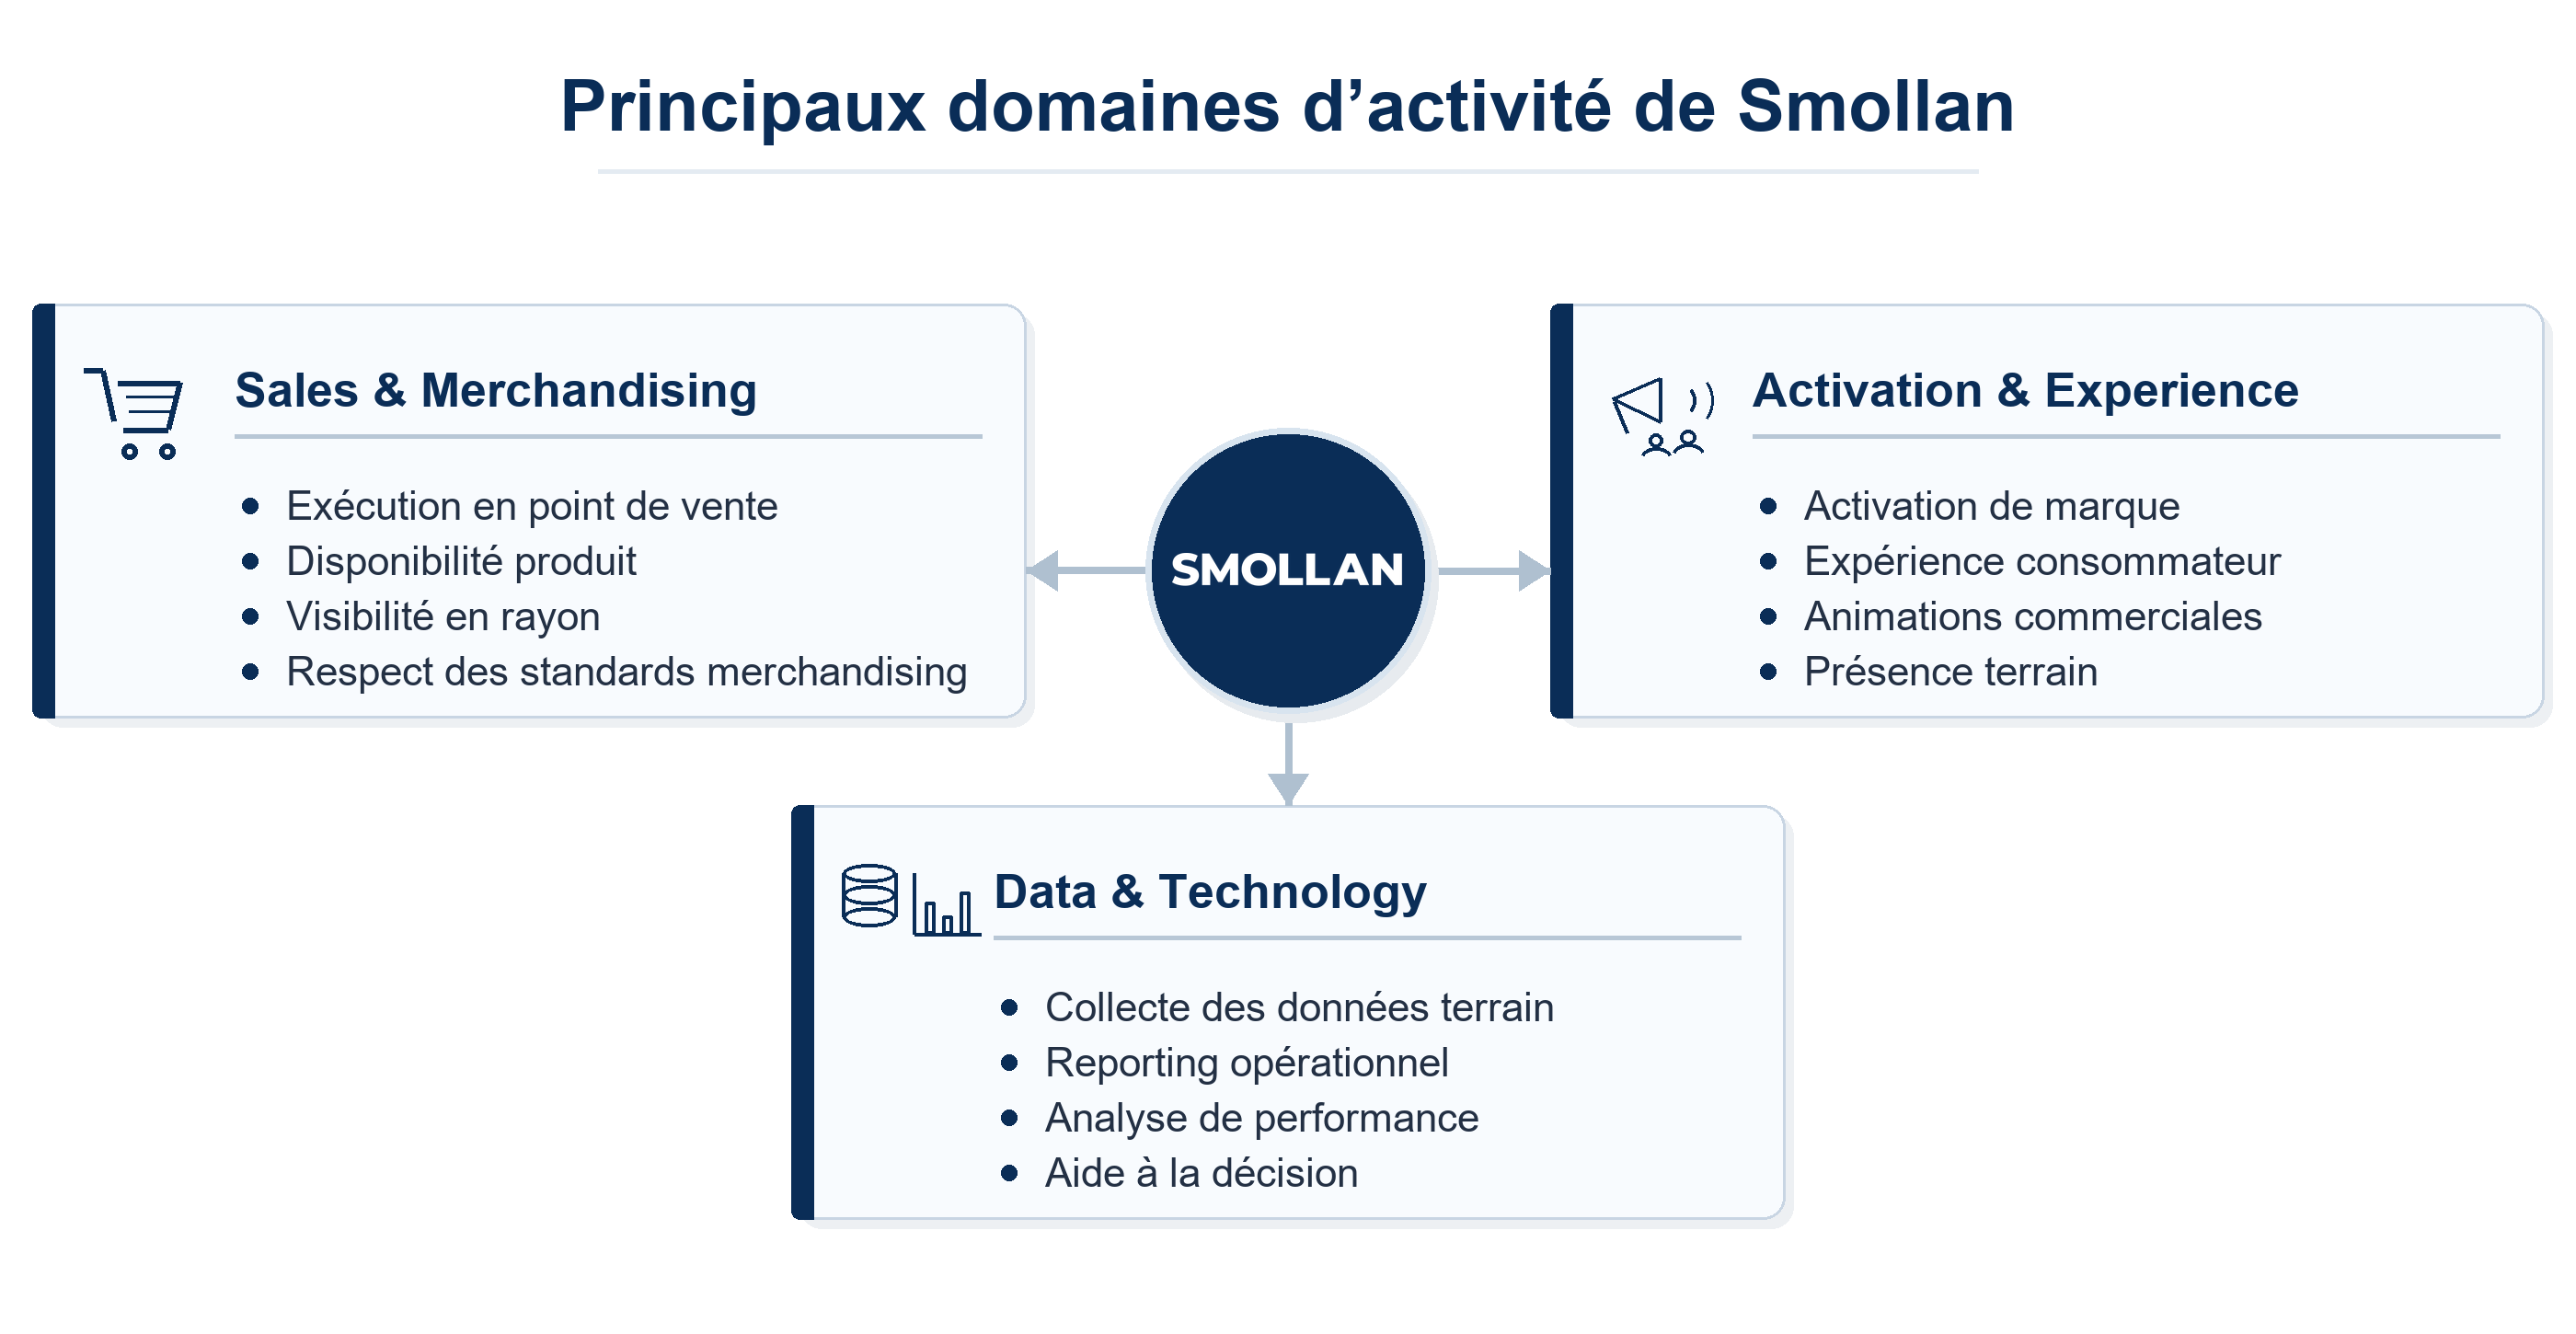
\includegraphics[width=\textwidth]{figures/architecture/smollan_activity_areas.png}
    \caption{Principaux domaines d’activité de Smollan}
    \label{fig:smollan-activity-areas}
\end{figure}

Ces domaines montrent que Smollan intervient à la fois dans l’exécution commerciale, l’activation des marques, la collecte d’informations terrain et l’analyse de la performance. Cette orientation explique le lien direct entre le contexte métier du stage et la mise en place d’une solution data-driven pour le suivi des activités terrain.

\subsection{Principaux clients et partenaires de Smollan}

Smollan accompagne différents types de marques, de distributeurs et de partenaires opérant dans des environnements commerciaux variés. Ces collaborations peuvent concerner les biens de grande consommation, les boissons, l’hygiène et les soins, la technologie, le retail ou encore l’agroalimentaire. L’objectif n’est pas de présenter une liste exhaustive de partenaires, mais de situer l’écosystème dans lequel les activités de Smollan s’inscrivent.

Dans le cadre de ce Projet de Fin d’Études, le périmètre étudié est centré sur les opérations de merchandising terrain liées au projet Unilever. Cette précision permet de distinguer l’écosystème général de Smollan du champ d’analyse réellement traité dans le rapport.

La figure suivante illustre l’écosystème général dans lequel s’inscrivent les activités de Smollan.

\begin{figure}[H]
    \centering
    
\includegraphics[width=0.45\textwidth]{SMOLLAN.png}
    \caption{Illustration de l’écosystème de partenaires et clients de Smollan}
    \label{fig:smollan-partners}
\end{figure}

Cette illustration accompagne la présentation de l’écosystème de Smollan, qui couvre différents secteurs d’activité et différents types de partenaires. Dans le cadre du présent rapport, le périmètre d’étude reste toutefois centré sur les opérations de merchandising liées au projet Unilever.

\subsection{Smollan Morocco}

Smollan Morocco représente la présence locale du groupe Smollan au Maroc. Elle accompagne plusieurs clients dans le suivi de leurs activités commerciales et merchandising, en s’appuyant sur des équipes terrain, des superviseurs et des outils de reporting opérationnel.

Dans ce contexte, les données collectées sur le terrain jouent un rôle important dans le pilotage quotidien des opérations. Elles permettent de suivre l’exécution des visites, la couverture des magasins, la disponibilité des produits, la qualité d’exécution et les indicateurs nécessaires à la prise de décision.

Le projet réalisé durant le stage s’intègre dans cette logique. Il vise à mieux exploiter les données issues du terrain afin de renforcer le suivi opérationnel, de structurer l’historique des informations et de proposer des supports de restitution adaptés aux différents utilisateurs.

\section{Présentation du client Unilever}

Unilever est une entreprise internationale opérant dans le secteur des biens de grande consommation. Ses activités couvrent plusieurs catégories de produits, notamment les soins personnels, l’hygiène, l’entretien de la maison, l’alimentation et d’autres produits utilisés quotidiennement par les consommateurs.

Dans le cadre des opérations de merchandising, Unilever accorde une importance particulière à la disponibilité de ses produits en magasin, à leur visibilité en rayon, au respect des standards d’exécution et à la qualité de la présence de ses marques dans les points de vente. Ces éléments sont essentiels pour soutenir la performance commerciale et assurer une meilleure expérience d’achat.

Le projet réalisé chez Smollan Morocco concerne le suivi des opérations de merchandising terrain liées au projet Unilever. Il vise à améliorer l’exploitation des données collectées en magasin afin de faciliter le pilotage, l’analyse et la consultation des informations d’exécution.

La figure suivante présente le logo du client concerné par le projet.

\begin{figure}[H]
    \centering
    
\includegraphics[width=0.28\textwidth]{Logo-blue-transparent-RGB.eps}
    \caption{Logo d’Unilever}
    \label{fig:logo-unilever}
\end{figure}

La présence du logo permet d’identifier le client autour duquel s’articulent les opérations de merchandising étudiées dans ce projet.

\section{Contexte métier du merchandising terrain}

Le merchandising terrain regroupe l’ensemble des actions réalisées en point de vente afin d’assurer la disponibilité, la visibilité et la bonne présentation des produits. Dans le cadre du projet Unilever, ces actions sont réalisées par des merchandisers qui effectuent des visites en magasin à l’aide de l’application Smart 3.

Lors de chaque visite, le merchandiser renseigne plusieurs informations relatives à l’exécution terrain. Ces informations peuvent concerner la disponibilité des produits, la qualité d’exécution, le respect du planogramme, le placement primaire ou secondaire, le SOS (\textit{Share of Shelf}), les relevés de prix, les photos justificatives ainsi que les données de localisation collectées par l’application.

Le suivi de ces opérations implique plusieurs niveaux d’exploitation. D’une part, les données saisies permettent d’assurer un suivi opérationnel interne, notamment pour vérifier l’avancement des visites, les écarts de couverture ou les situations nécessitant une justification. D’autre part, certaines informations sont utilisées pour préparer des reportings destinés au client, notamment autour de la disponibilité produit, de la qualité d’exécution ou de la visibilité en rayon.

Dans ce contexte, la donnée terrain devient un élément central du pilotage. Elle ne sert pas uniquement à constater qu’une visite a été réalisée, mais permet également d’analyser la qualité de l’exécution, de suivre les performances opérationnelles et d’améliorer la visibilité des différents acteurs sur l’activité en magasin.

La figure suivante présente une vue simplifiée des principaux acteurs et flux métier liés aux opérations de merchandising terrain.

\begin{figure}[H]
    \centering
    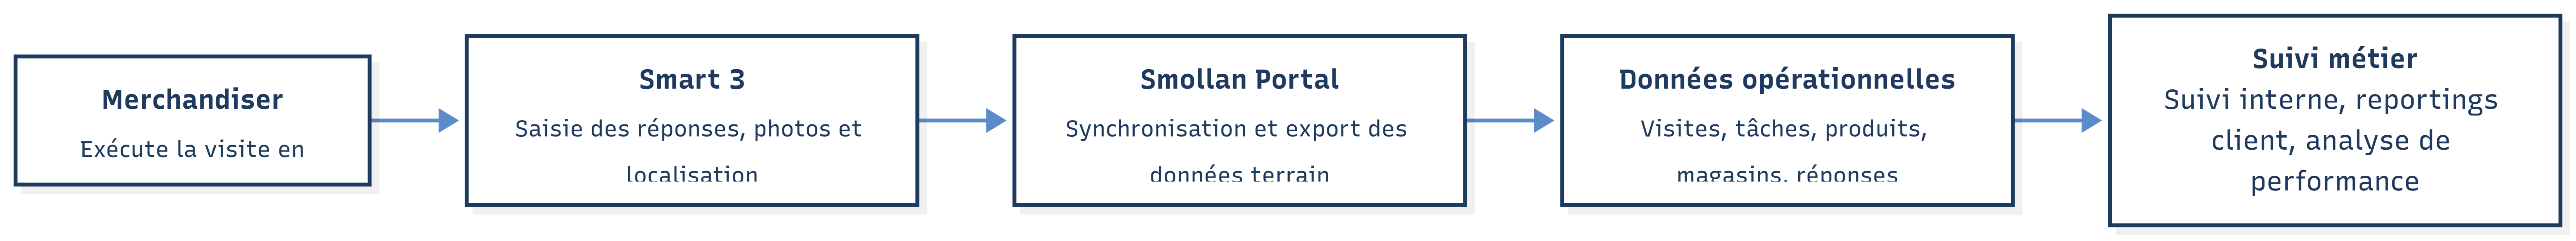
\includegraphics[width=0.9\textwidth]{figures/architecture/flux_metier_merchandising.png}
    \caption{Acteurs et flux métier des opérations de merchandising terrain}
    \label{fig:business-context-flow}
\end{figure}

Ce schéma montre que les informations collectées en magasin constituent la base du suivi opérationnel. Elles sont saisies dans l'application Smart 3, synchronisées vers le portail Smollan, puis exploitées pour alimenter le suivi interne et les reportings destinés au client.

\section{Problématique}

Le suivi des opérations terrain du projet Unilever repose sur des données collectées quotidiennement à travers l’application Smart 3, puis exportées depuis le portail Smollan sous forme de fichiers Excel. Ces fichiers contiennent une quantité importante d’informations relatives aux visites, aux magasins, aux merchandisers, aux produits et aux tâches exécutées.

Cependant, l’exploitation de ces données devient complexe lorsque les informations sont dispersées entre plusieurs fichiers et reportings. Le fichier \textit{Data Dump} apporte le détail des réponses terrain, tandis que le fichier \textit{Coverage} permet de suivre les visites planifiées, réalisées, rejetées, déviées ou non effectuées. Cette séparation nécessite un travail de structuration afin d’obtenir une vision cohérente, fiable et exploitable des opérations.

Par ailleurs, les besoins de restitution ne sont pas identiques selon les utilisateurs. Le management et les équipes internes ont besoin d’indicateurs consolidés pour le pilotage et le contrôle opérationnel, tandis que les superviseurs côté client doivent disposer d’une consultation plus ciblée sur les magasins qui leur sont affectés. Les situations nécessitant une validation ou une vérification interne doivent, quant à elles, être traitées dans un espace back-office adapté.

La problématique du projet peut donc être formulée comme suit :

\begin{quote}
Comment concevoir une solution data-driven permettant de centraliser et structurer les données de merchandising terrain du projet Unilever, afin de proposer des restitutions adaptées au pilotage interne, à la consultation client et au suivi des validations opérationnelles ?
\end{quote}

\section{Objectifs du projet}

L’objectif général du projet est de concevoir une solution data-driven permettant d’améliorer le suivi et l’analyse des opérations de merchandising terrain du projet Unilever chez Smollan Morocco.

Pour atteindre cet objectif, plusieurs objectifs spécifiques ont été définis :

\begin{itemize}
    \item mettre en place un pipeline ETL permettant d’extraire, transformer et charger les données issues des fichiers \textit{Data Dump} et \textit{Coverage} ;
    \item centraliser les données dans une base MySQL afin de structurer l’historique des visites, des magasins, des merchandisers, des produits et des tâches exécutées ;
    \item concevoir des tableaux de bord Power BI permettant de suivre les indicateurs opérationnels et d’accompagner le pilotage interne ;
    \item développer une application mobile orientée client permettant aux superviseurs Unilever de consulter uniquement les magasins qui leur sont affectés ;
    \item mettre en place un portail back-office interne destiné à l’analyse des validations opérationnelles et des situations nécessitant une vérification ;
    \item préparer une architecture évolutive pouvant intégrer progressivement de nouvelles règles de validation, de nouvelles vues analytiques et de nouvelles sources de données.
\end{itemize}

Ces objectifs traduisent la volonté de passer d’une exploitation principalement basée sur des fichiers et reportings séparés vers une solution structurée, centralisée et adaptée aux différents usages métier.

\section{Méthodologie de travail}

\subsection{Démarche adoptée}

La réalisation du projet a été conduite selon une démarche progressive et itérative. Cette approche a permis de partir de la compréhension du contexte métier avant de passer à l’analyse des données, à la conception de la solution, au développement des différentes couches et aux ajustements nécessaires.

La première étape a consisté à comprendre le fonctionnement opérationnel du projet Unilever. Cette phase a porté sur l’identification des acteurs impliqués, des outils utilisés sur le terrain, des types de visites réalisées, ainsi que des reportings produits à partir des données collectées. Elle a permis de mieux cerner le rôle des données dans le suivi quotidien des opérations.

La deuxième étape a concerné l’analyse des sources de données disponibles, notamment les fichiers \textit{Data Dump} et \textit{Coverage}. L’objectif était de comprendre la structure de ces fichiers, la signification des champs, leur complémentarité et leur potentiel d’exploitation pour le suivi opérationnel et analytique.

La troisième étape a porté sur la conception progressive de la solution. Le travail a été organisé par couches fonctionnelles, en commençant par la structuration des données, puis la restitution analytique, avant d’aborder les interfaces de consultation et de validation. Cette organisation a permis de garder une cohérence entre les besoins métier et les choix techniques.

La dernière étape a été consacrée aux tests, aux ajustements et à la documentation. Les résultats obtenus ont été vérifiés à partir des données réelles afin de contrôler la cohérence des indicateurs, la fiabilité des transformations et l’utilité des restitutions proposées. La rédaction du rapport a été menée en parallèle avec l’avancement du projet afin de documenter progressivement le contexte, les choix effectués, les résultats obtenus, les limites rencontrées et les perspectives d’amélioration.

\subsection{Phases du projet}

Afin de structurer le travail, le projet a été organisé en plusieurs phases complémentaires. Ces phases ne correspondent pas uniquement à des livrables attendus, mais décrivent l’ordre dans lequel les activités ont été conduites : cadrage métier, analyse des fichiers, conception du pipeline, centralisation des données, restitution analytique, développement applicatif, puis tests et documentation.

La figure suivante synthétise les principales étapes de la démarche adoptée durant le projet.

\begin{figure}[H]
    \centering
    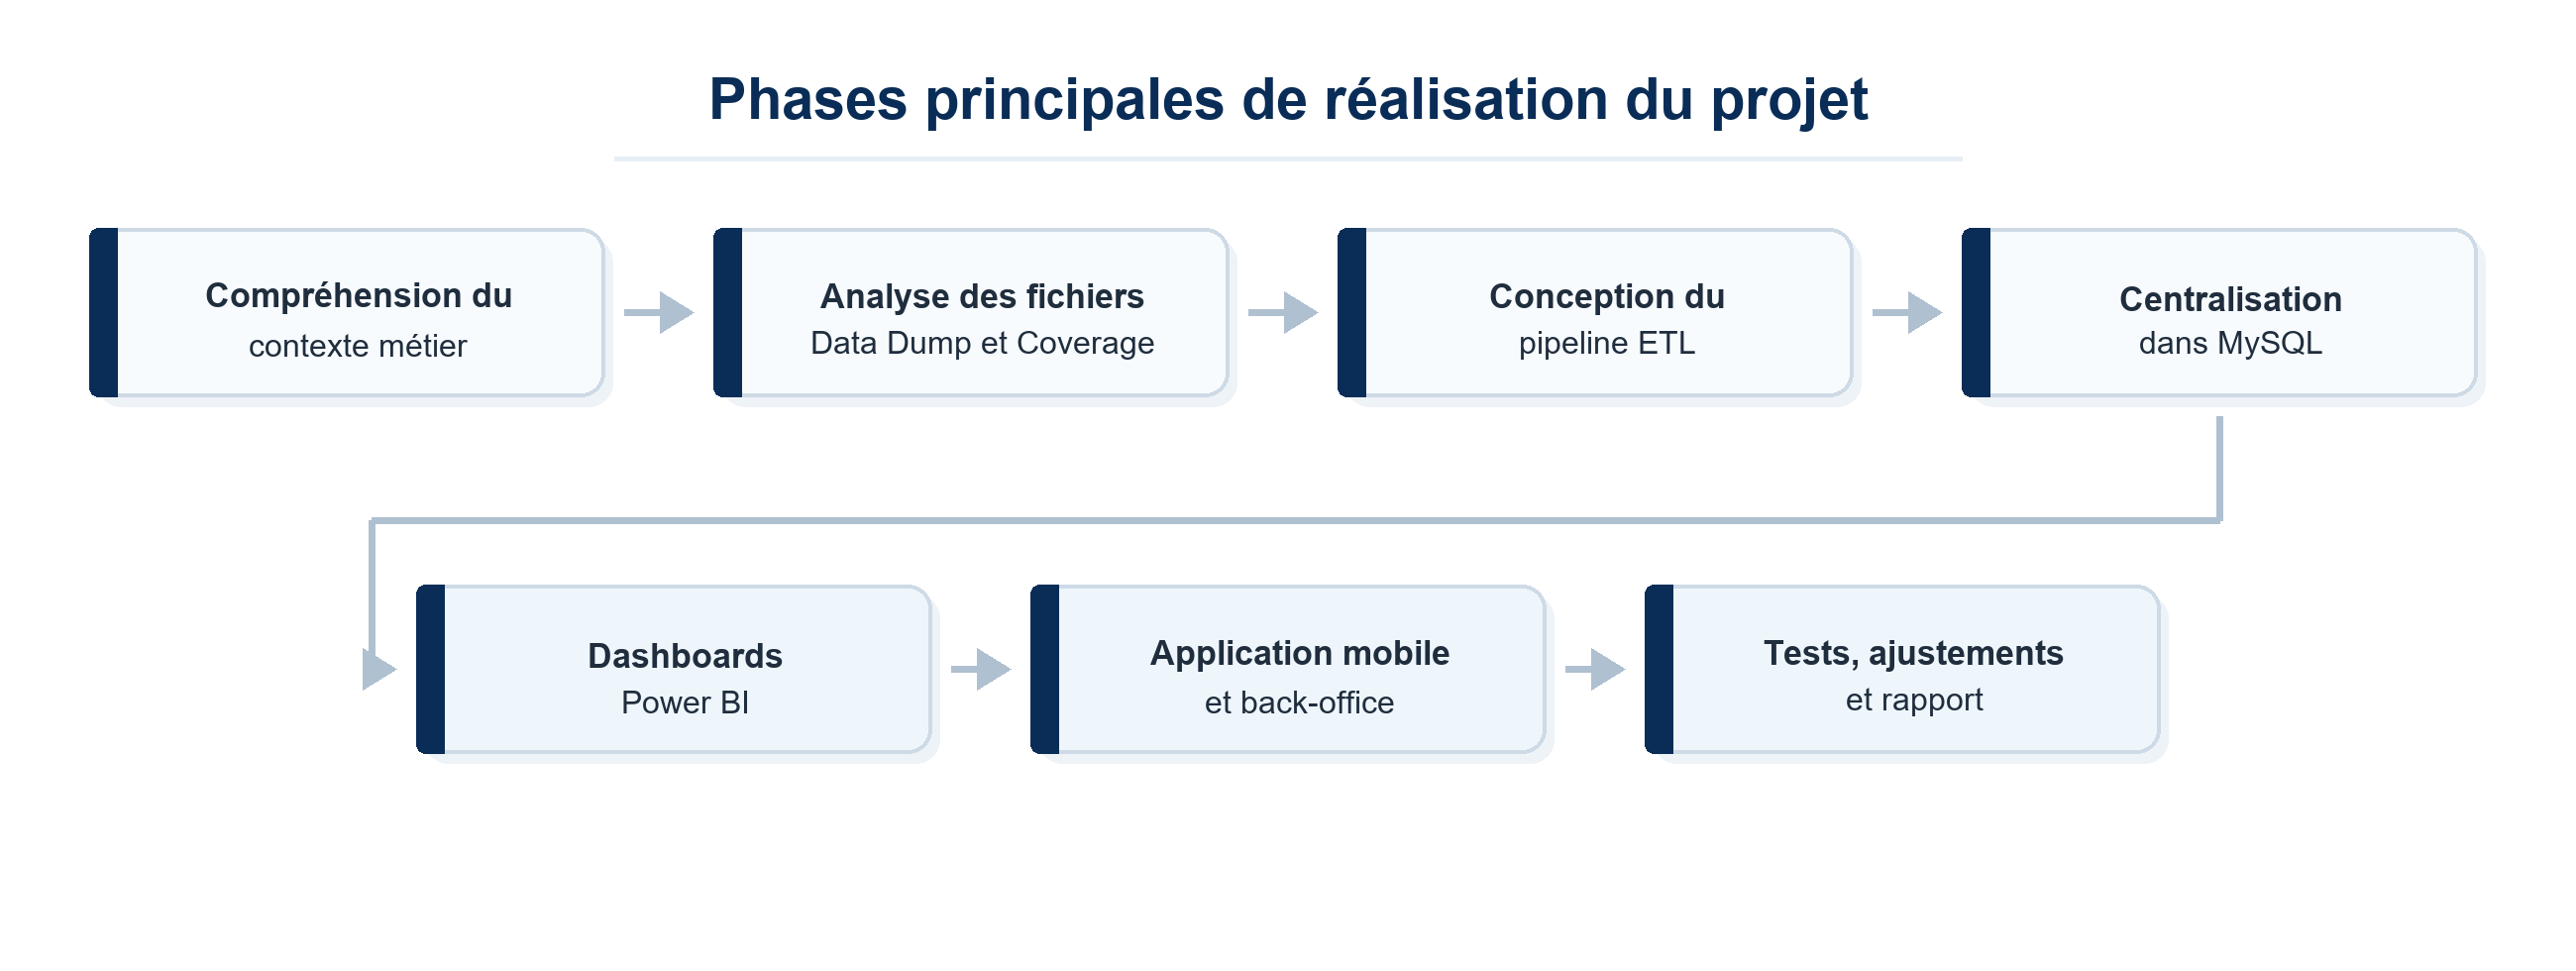
\includegraphics[width=0.95\textwidth]{figures/architecture/project_phases.png}
    \caption{Phases principales de réalisation du projet}
    \label{fig:project-phases}
\end{figure}

Cette organisation met en évidence la logique de progression adoptée. Les premières phases ont permis de comprendre le besoin et de structurer les données, tandis que les phases suivantes ont porté sur la restitution, les interfaces de consultation et les ajustements nécessaires à partir des résultats observés.

\subsection{Planification du projet}

La planification du projet doit permettre de situer les principales étapes de travail dans le temps. Elle repose sur une progression structurée depuis le cadrage métier jusqu’aux tests et à la rédaction du rapport.

La figure suivante accompagne la présentation de la planification générale du projet.

\begin{figure}[H]
    \centering
    
\includegraphics[width=0.45\textwidth]{SMOLLAN.png}
    \caption{Illustration de la planification générale du projet}
    \label{fig:gantt-pfe}
\end{figure}

La planification du projet couvre les principales étapes de réalisation, depuis la compréhension du contexte métier jusqu’aux tests et à la rédaction du rapport. Elle inclut notamment l’analyse des fichiers Data Dump et Coverage, la conception du pipeline ETL, la centralisation des données, la réalisation des tableaux de bord, le développement des interfaces applicatives et les ajustements réalisés au cours du stage.

\section{Conclusion}

Ce chapitre a présenté le cadre général du Projet de Fin d’Études, en introduisant l’organisme d’accueil, le client Unilever ainsi que le contexte métier du merchandising terrain. Il a également permis de formuler la problématique du projet et de préciser les objectifs poursuivis.

Le projet s’inscrit dans une démarche de valorisation des données terrain, visant à mieux structurer les informations issues des opérations de merchandising et à proposer des outils adaptés aux besoins des différents utilisateurs. Le chapitre suivant sera consacré à l’analyse de l’existant et des besoins, afin de détailler le fonctionnement actuel du processus et les limites qui justifient la solution proposée.
